\documentclass[landscape]{article}
\usepackage[a4paper,landscape,margin=1.5cm]{geometry}
\usepackage{graphicx}
\usepackage{array}
\usepackage{tabularx}
\usepackage{colortbl}
\usepackage{xcolor}
\usepackage{fancyhdr}
\usepackage{tikz}
\usepackage{booktabs}
\usepackage{subcaption}
\usepackage{pagecolor}
\usepackage{multirow}
\usepackage{lastpage}
\usepackage{tgheros} % Modern sans-serif font
\usepackage{setspace}
\usepackage[T1]{fontenc}
\usepackage{makecell}
\usepackage{enumitem} % Better list control
\usepackage{fontawesome5} % For icons
\usepackage{pdflscape} % Better landscape handling

\graphicspath{{illustration/}{reference/}{figures/}}  % Paths for images

% Define refined color palette
\definecolor{primaryblue}{RGB}{41, 65, 94}   % Deeper blue for main headers
\definecolor{secondaryblue}{RGB}{78, 112, 155} % Lighter blue for secondary elements
\definecolor{lightblue}{RGB}{235, 242, 250} % Very light blue for table backgrounds
\definecolor{mediumblue}{RGB}{120, 150, 180} % Medium blue for table headers
\definecolor{accentgold}{RGB}{216, 181, 109} % Gold accent color
\definecolor{backgroundbeige}{RGB}{252, 250, 245} % Light beige background
\definecolor{tablehead}{RGB}{245, 245, 245} % Subtle gray for table headers
\definecolor{bordercolor}{RGB}{220, 220, 220} % Subtle border color
\definecolor{subtleshadow}{RGB}{240, 240, 240} % For subtle shadows

% Set background color
\pagecolor{white}

% Set document font to sans-serif
\renewcommand{\familydefault}{\sfdefault}

% Better spacing
\setstretch{1.2}
\setlength{\parindent}{0pt}
\setlength{\parskip}{8pt}
\renewcommand{\arraystretch}{1.5} % Improve table row height globally

% Fix for table line alignment
\setlength{\arrayrulewidth}{0.5pt}
\setlength{\tabcolsep}{6pt}

% Custom page style
\pagestyle{fancy}
\fancyhf{}
\renewcommand{\headrulewidth}{0pt}
\renewcommand{\footrulewidth}{0pt}

% Enhanced Header with brand bar and subtle shadow
\fancyhead[C]{%
\begin{tikzpicture}[remember picture, overlay]
    % Shadow effect
    \fill[subtleshadow] 
        ([yshift=-1.2cm, xshift=0.2cm]current page.north west) rectangle 
        ([yshift=-0.8cm, xshift=0.2cm]current page.north east);
    
    % Header bar with gradient
    \shade[top color=primaryblue, bottom color=secondaryblue] 
        ([yshift=-1cm]current page.north west) rectangle 
        ([yshift=0cm]current page.north east);
    
    % Gold accent line
    \fill[accentgold] 
        ([yshift=-1cm]current page.north west) rectangle 
        ([yshift=-0.9cm]current page.north east);
    
    % Brand name with logo placeholder
    \node[anchor=west, text=white, font=\Large\bfseries] 
        at ([xshift=1cm, yshift=-0.5cm]current page.north west) 
        {J.LINDEBERG};
    
    % Document type indicator
    \node[anchor=east, text=white, font=\large] 
        at ([xshift=-1cm, yshift=-0.5cm]current page.north east) 
        {TECHNICAL SPECIFICATION};
\end{tikzpicture}%
}

% Enhanced footer with contact info and modern design
\fancyfoot[C]{%
\begin{tikzpicture}[remember picture, overlay]
    % Shadow effect
    \fill[subtleshadow] 
        ([yshift=0.9cm, xshift=0.2cm]current page.south west) rectangle 
        ([yshift=0.2cm, xshift=0.2cm]current page.south east);
    
    % Blue footer bar with gradient
    \shade[bottom color=primaryblue, top color=secondaryblue] 
        ([yshift=0.7cm]current page.south west) rectangle 
        ([yshift=0cm]current page.south east);
    
    % Gold accent line
    \fill[accentgold] 
        ([yshift=0.7cm]current page.south west) rectangle 
        ([yshift=0.65cm]current page.south east);
    
    % Copyright text with icon
    \node[anchor=west, text=white, font=\small] 
        at ([xshift=1cm, yshift=0.35cm]current page.south west) 
        {\faIcon{copyright} J.Lindeberg 2025};
    
    % Page number with icon
    \node[anchor=east, text=white, font=\small] 
        at ([xshift=-1cm, yshift=0.35cm]current page.south east) 
        {\faIcon{file-alt} PAGE \thepage\ OF \pageref{LastPage}};
\end{tikzpicture}%
}

% Improved section command with shadow effect
\newcommand{\techsection}[1]{%
\noindent\begin{tabularx}{\textwidth}{|X|}
\hline
\cellcolor{primaryblue}\textcolor{white}{\large\textbf{\faIcon{angle-right} #1}} \\
\hline
\end{tabularx}
\vspace{0.1cm}
}

% Command for elevated panels with shadow
\newcommand{\elevatedbox}[1]{%
\begin{tikzpicture}
\node[draw=bordercolor, line width=0.5pt, inner sep=10pt, fill=white, rounded corners=3pt, 
      drop shadow={shadow xshift=1pt, shadow yshift=-1pt, opacity=0.2}] {#1};
\end{tikzpicture}
}

\begin{document}

% Title with enhanced decorative elements and subtle shadow
\begin{center}

\begin{tikzpicture}
% Shadow layer
\node[inner sep=12pt, opacity=0.1, yshift=-2pt, xshift=2pt] (shadow) {\Huge\textbf{\textcolor{black}{Technical Specification Sheet}}};
% Main title
\node[inner sep=12pt] (title) {\Huge\textbf{\textcolor{primaryblue}{Technical Specification Sheet}}};
% Dual accent lines
\draw[accentgold, line width=2pt] ([yshift=-5pt]title.south west) -- ([yshift=-5pt]title.south east);
\draw[secondaryblue, line width=1pt] ([yshift=-9pt]title.south west) -- ([yshift=-9pt]title.south east);
% Icon decorations on both sides
\node[anchor=east, xshift=-10pt] at (title.west) {\textcolor{accentgold}{\Large\faIcon{ruler}}};
\node[anchor=west, xshift=10pt] at (title.east) {\textcolor{accentgold}{\Large\faIcon{cut}}};
\end{tikzpicture}
\end{center}

\vspace{0.5cm}

% PRODUCT DETAILS - Enhanced with icons and better layout
\begin{center}
\begin{tabular}{|>{\bfseries\raggedright\arraybackslash}p{3.2cm}|p{4cm}|>{\bfseries\raggedright\arraybackslash}p{3.2cm}|p{4cm}|}
\hline
\rowcolor{tablehead}\faIcon{tag} Brand: & J.Lindeberg & \rowcolor{tablehead}\faIcon{user} Designer: & John \\
\hline
\faIcon{tshirt} Style Name: & Leather Bomber Jacket & \faIcon{hashtag} Style Number: & JL-001 \\
\hline
\rowcolor{tablehead}\faIcon{layer-group} Category: & Outerwear & \rowcolor{tablehead}\faIcon{calendar-alt} Season: & Fall/Winter 2025 \\
\hline
\faIcon{calendar-day} Date: & October 5, 2023 & \faIcon{code-branch} Version: & V1.0 \\
\hline
\end{tabular}
\end{center}

\vspace{0.5cm}

% PRODUCT DESCRIPTION with elevated design
\begin{center}
\begin{tabular}{|p{14cm}|}
\hline
\rowcolor{tablehead}\multicolumn{1}{|c|}{\textbf{\faIcon{info-circle} PRODUCT DESCRIPTION}} \\
\hline
\vspace{0.2cm}
\large This jacket takes inspiration from classic bomber silhouettes while integrating the sleek and refined details seen in the reference image. The front showcases large flap pockets and a structured ribbed collar, while the back remains simplified with subtle panel lines for a contemporary look. Crafted in high-quality leather, it offers both durability and a polished finish. Its lightly padded interior and ribbed trims at the cuffs and hem ensure warmth and a comfortable fit. Overall, the piece embodies a modern fusion of timeless style with premium materials. 
\vspace{0.3cm} \\
\hline
\end{tabular}
\end{center}

\newpage

% --------------------------------- FRONT VIEW SECTION ---------------------------------
\techsection{FRONT VIEW}
\vspace{-0.3cm}

\begin{tabular}{p{0.49\textwidth}|p{0.49\textwidth}}
% Left side - FRONT VIEW with better frame
\begin{center}
\begin{tikzpicture}
\node[draw=bordercolor, line width=0.5pt, inner sep=4pt, fill=white, rounded corners=3pt]{
    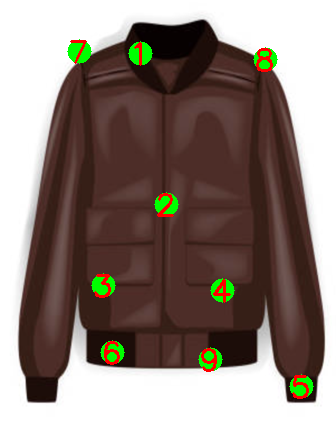
\includegraphics[width=0.35\textwidth,height=12cm,keepaspectratio]{jacket_front.png}
};
% Add a small label on top
\node[anchor=north, fill=accentgold, text=white, font=\small\bfseries, rounded corners=2pt, inner sep=2pt]
    at ([yshift=0.5cm]current bounding box.north) {FRONT VIEW};
\end{tikzpicture}
\end{center}
&
% Right side - Attributes Table FRONT VIEW with improved formatting
\begin{center}
\begin{tabular}{|>{\columncolor{lightblue}\bfseries}p{3.5cm}|p{7cm}|}
\hline
\rowcolor{mediumblue}\multicolumn{1}{|c|}{\textcolor{white}{\textbf{\faIcon{list} Component}}} & \multicolumn{1}{c|}{\textcolor{white}{\textbf{\faIcon{info} Specifications}}} \\ \hline
1 - Ribbed Collar & The collar is crafted with a soft, ribbed knit to provide comfort and maintain shape. Reinforced stitching is used along the neckline to ensure long-term durability.\\ \hline
2 - Front Chest Panel & The front chest panel features a smooth, padded interior for insulation. It is top-stitched with matching thread for a neat, uniform finish.\\ \hline
3 - Left Pocket & A spacious flap pocket on the left side allows for convenient storage. The pocket flap is interfaced to maintain crisp edges and prevent sagging.\\ \hline
4 - Right Pocket & The right pocket replicates the left in size and style. Each pocket piece is double-stitched at stress points to prevent tearing.\\ \hline
5 - Right Cuff & The cuff uses stretch-resistant elastic to preserve its shape. Each cuff is attached with a snug overlock seam for a secure and comfortable fit.\\ \hline
6 - Left Waist Panel & The left waist area is reinforced with an inner facing. This helps prevent wrinkles and ensures the jacket retains a clean silhouette.\\ \hline
7 - Left Shoulder & The left shoulder seam is slightly padded for structure. Additional seam binding is applied to reduce friction and ensure a smooth inside finish.\\ \hline
8 - Right Shoulder & The right shoulder mirrors the left in construction. A lightweight foam padding shapes the shoulder line for a balanced appearance.\\ \hline
9 - Waistband & The ribbed waistband is designed to hug the body securely. A heavier rib knit is employed here to maintain stretch recovery over time.\\ \hline
\end{tabular}
\end{center}
\end{tabular}

\vspace{0.5cm}

% MEASUREMENTS TABLE FRONT VIEW - WITH IMPROVED STYLING
\noindent\begin{tabularx}{\textwidth}{|>{\columncolor{lightblue}\bfseries}X|X|>{\centering\arraybackslash}X|>{\centering\arraybackslash}X|>{\centering\arraybackslash}X|>{\centering\arraybackslash}X|}
\hline
\rowcolor{primaryblue}\multicolumn{6}{|c|}{\textcolor{white}{\large\textbf{\faIcon{ruler-combined} FRONT MEASUREMENTS}}} \\
\hline
\rowcolor{mediumblue}\textcolor{white}{\textbf{Measurement}} & \textcolor{white}{\textbf{Description}} & \textcolor{white}{\textbf{XS}} & \textcolor{white}{\textbf{S}} & \textcolor{white}{\textbf{M}} & \textcolor{white}{\textbf{L}} \\ \hline
Shoulder Width & Measured between the armhole seams at the front. & 38 cm & 40 cm & 42 cm & 44 cm \\ \hline
Chest Width & Taken across the fullest part of the front chest. & 48 cm & 50 cm & 52 cm & 54 cm \\ \hline
Waist Circumference & Measured around the lower ribbed waistband at the front. & 88 cm & 92 cm & 96 cm & 100 cm \\ \hline
Sleeve Length & From shoulder seam to cuff edge along the outer arm. & 61 cm & 62 cm & 63 cm & 64 cm \\ \hline
Front Length & From highest shoulder point down to the waistband. & 58 cm & 60 cm & 62 cm & 64 cm \\ \hline
Collar Circumference & Around the base of the ribbed collar at front. & 38 cm & 39 cm & 40 cm & 41 cm \\ \hline
\end{tabularx}
% ---------------------------------------------------------------------------------------------
\newpage

% --------------------------------- BACK VIEW SECTION ---------------------------------
\techsection{BACK VIEW}
\vspace{-0.3cm}

\begin{tabular}{p{0.49\textwidth}|p{0.49\textwidth}}
% Left side - BACK VIEW with better frame
\begin{center}
\begin{tikzpicture}
\node[draw=bordercolor, line width=0.5pt, inner sep=4pt, fill=white, rounded corners=3pt]{
    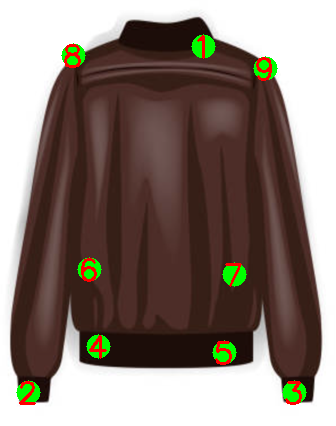
\includegraphics[width=0.35\textwidth,height=12cm,keepaspectratio]{jacket_back.png}
};
% Add a small label on top
\node[anchor=north, fill=accentgold, text=white, font=\small\bfseries, rounded corners=2pt, inner sep=2pt]
    at ([yshift=0.5cm]current bounding box.north) {BACK VIEW};
\end{tikzpicture}
\end{center}
&
% Right side - Attributes Table BACK VIEW with improved formatting
\begin{center}
\begin{tabular}{|>{\columncolor{lightblue}\bfseries}p{3.5cm}|p{7cm}|}
\hline
\rowcolor{mediumblue}\multicolumn{1}{|c|}{\textcolor{white}{\textbf{\faIcon{list} Component}}} & \multicolumn{1}{c|}{\textcolor{white}{\textbf{\faIcon{info} Specifications}}} \\ \hline
1 - Back Collar & The back collar is seamlessly connected to the front collar ribbing. It is lightly padded for extra comfort at the neckline.\\ \hline
2 - Upper Back Yoke & A shaped back yoke introduces a slight curve for better fit. Double-layer interfacing helps retain the jacket’s structure.\\ \hline
3 - Left Side Seam & The left side seam is reinforced with a top stitch. This helps prevent fraying and maintains clean lines down the back.\\ \hline
4 - Right Side Seam & Mirroring the left side, it features identical reinforcement. Additional bar tacks are placed at high-stress areas near the underarm.\\ \hline
5 - Right Hem Edge & The lower right hem transitions into the waistband smoothly. A secure overlock stitch prevents the edge from unraveling.\\ \hline
6 - Left Sleeve Panel & The sleeve panel is attached with flat-felled seams to reduce bulk. It aligns precisely with the armhole for comfortable movement.\\ \hline
7 - Right Sleeve Panel & Identical to the left, this panel uses matching thread for consistency. The seam construction resists wear in rigorous use.\\ \hline
8 - Left Shoulder Curve & This shoulder curve is gently tailored for a natural drape. Extra stitching ensures the seam stays smooth under tension.\\ \hline
9 - Right Shoulder Curve & The right shoulder curve is cut to match the left for balance. Reinforcement tape is used along the seam to minimize stretching.\\ \hline
\end{tabular}
\end{center}
\end{tabular}

\vspace{0.5cm}

% MEASUREMENTS TABLE BACK VIEW - WITH IMPROVED STYLING
\noindent\begin{tabularx}{\textwidth}{|>{\columncolor{lightblue}\bfseries}X|X|>{\centering\arraybackslash}X|>{\centering\arraybackslash}X|>{\centering\arraybackslash}X|>{\centering\arraybackslash}X|}
\hline
\rowcolor{primaryblue}\multicolumn{6}{|c|}{\textcolor{white}{\large\textbf{\faIcon{ruler-combined} BACK MEASUREMENTS}}} \\
\hline
\rowcolor{mediumblue}\textcolor{white}{\textbf{Measurement}} & \textcolor{white}{\textbf{Description}} & \textcolor{white}{\textbf{XS}} & \textcolor{white}{\textbf{S}} & \textcolor{white}{\textbf{M}} & \textcolor{white}{\textbf{L}} \\ \hline
Back Length & From collar seam down to the bottom of the waistband. & 60 cm & 62 cm & 64 cm & 66 cm \\ \hline
Across Shoulders & Measured from left shoulder curve to right shoulder curve. & 40 cm & 42 cm & 44 cm & 46 cm \\ \hline
Armhole Depth & The vertical measurement from top shoulder seam to underarm. & 24 cm & 25 cm & 26 cm & 27 cm \\ \hline
Sleeve Length (Back) & From back shoulder seam to the cuff edge along the backside. & 62 cm & 63 cm & 64 cm & 65 cm \\ \hline
Back Waist Width & Measured across the narrowest point of the waist at the back. & 46 cm & 48 cm & 50 cm & 52 cm \\ \hline
Shoulder Drop & The slope from the collar to where the sleeve attaches. & 13 cm & 14 cm & 15 cm & 16 cm \\ \hline
\end{tabularx}
% ---------------------------------------------------------------------------------------------

\newpage

% REFERENCE IMAGES SECTION with callouts
\techsection{REFERENCE}
\vspace{-0.3cm}

\begin{tabular}{p{0.49\textwidth}|p{0.49\textwidth}}
% Left side - Place reference images with annotations
\begin{center}
\begin{tikzpicture}
\node[draw=bordercolor, line width=0.5pt, inner sep=4pt, fill=white, rounded corners=3pt] (img) {
    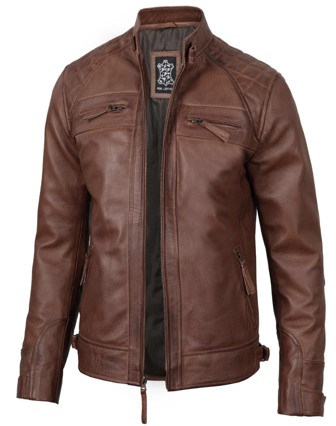
\includegraphics[width=0.35\textwidth,height=12cm,keepaspectratio]{jacket_reference.png}
};

% Add a small label on top
\node[anchor=north, fill=accentgold, text=white, font=\small\bfseries, rounded corners=2pt, inner sep=2pt] 
    at ([yshift=0.5cm]current bounding box.north) {INSPIRATION \& DETAILS};
\end{tikzpicture}
\end{center}
&
% Right side - Description of reference image with enhanced formatting
\begin{center}
\begin{tabular}{|p{10cm}|}
\hline
\rowcolor{mediumblue}\multicolumn{1}{|c|}{\textcolor{white}{\textbf{\faIcon{lightbulb} Design Inspiration \& Notes}}} \\
\hline
\begin{minipage}[t]{\linewidth}
\vspace{0.3cm}
This reference image highlights a clean, modern silhouette with a slightly fitted cut. It showcases a balanced collar shape and pocket placement that informs the final design. 
\begin{itemize}[leftmargin=*, label={\textcolor{accentgold}{\faIcon{check-circle}}}]
  \item Premium leather finish with subtle sheen
  \item Streamlined zipper detailing
  \item Minimal top-stitched accents
\end{itemize}
\vspace{0.3cm}
\end{minipage} \\
\hline
\end{tabular}
\end{center}
\end{tabular}

\newpage

% BILL OF MATERIALS with enhanced design
\techsection{BILL OF MATERIALS}
\vspace{-0.3cm}
\noindent\begin{tabularx}{\textwidth}{|>{\columncolor{lightblue}\bfseries}p{3cm}|X|>{\raggedleft\arraybackslash}p{2.5cm}|>{\raggedleft\arraybackslash}p{2.5cm}|}
\hline
\rowcolor{mediumblue}\textcolor{white}{\textbf{Material}} & \textcolor{white}{\textbf{Description}} & \textcolor{white}{\textbf{Unit Cost}} & \textcolor{white}{\textbf{Total Cost}} \\
\hline
Leather Shell & Full-grain cow leather, 1.2 mm thickness & \$50.00/yd & \$150.00 \\
\hline
Lining & Polyester lining, satin finish & \$5.00/yd & \$15.00 \\
\hline
Ribbing & Cotton-nylon blend for collar/cuffs & \$3.00/yd & \$6.00 \\
\hline
Zipper & Heavy-duty metal YKK & \$2.50/ea & \$2.50 \\
\hline
Interfacing & Fusible for structural areas & \$1.00/yd & \$2.00 \\
\hline
Thread & Polyester, color matched & \$0.50/spool & \$0.50 \\
\hline
Snaps & Brass snaps for closures & \$0.20/ea & \$1.00 \\
\hline
Label & Brand label and size tag & \$0.50/ea & \$0.50 \\
\hline
\multicolumn{3}{|r|}{\textbf{Total Material Cost:}} & \$177.50 \\
\hline
\end{tabularx}

\vspace{0.7cm}

\newpage

% CARE INSTRUCTIONS with icons
\techsection{CARE INSTRUCTIONS}
\vspace{-0.3cm}

\noindent\begin{tabularx}{\textwidth}{|X|}
\hline
\begin{minipage}[t]{\linewidth}
\vspace{0.3cm}
\large For best long-term maintenance of this leather jacket, please follow these guidelines:
\begin{itemize}
\item Store in a cool, dry environment, and avoid direct sunlight or damp areas.
\item Gently wipe dirt with a soft cloth; do not soak or scrub.
\item Apply a suitable leather conditioner periodically to preserve suppleness.
\end{itemize}

\begin{center}
\begin{tabular}{ccccc}
\textcolor{primaryblue}{\Large\faIcon{ban}} &
\textcolor{primaryblue}{\Large\faIcon{ban}} &
\textcolor{primaryblue}{\Large\faIcon{ban}} &
\textcolor{primaryblue}{\Large\faIcon{ban}} &
\textcolor{primaryblue}{\Large\faIcon{check-circle}} \\
No Machine Wash & No Bleach & No Tumble Dry & No Iron & Professional Leather Clean \\
\end{tabular}
\end{center}

\vspace{0.3cm}
\end{minipage} \\
\hline
\end{tabularx}

\vspace{0.7cm}

% ADDITIONAL COMMENTS with improved formatting
\techsection{ADDITIONAL COMMENTS}
\vspace{-0.3cm}
\noindent\begin{tabularx}{\textwidth}{|X|}
\hline
\begin{minipage}[t]{\linewidth}
\vspace{0.3cm}
\large 
% ADDITIONAL COMMENT HERE
\vspace{0.3cm}
\end{minipage} \\
\hline
\end{tabularx}

\vspace{0.7cm}
% SIGNATURES
\techsection{SIGNATURES}
\vspace{-0.3cm}
\noindent\begin{tabularx}{\textwidth}{|X|}
\hline
\begin{minipage}[t]{\linewidth}
\vspace{0.3cm}
\large\textbf{Approvals:} \underline{\hspace{5cm}} (Design Director) \hspace{1cm} \underline{\hspace{5cm}} (Production Manager)
\vspace{0.3cm}
\end{minipage} \\
\hline
\end{tabularx}

\newpage

% DISCLAIMER AND CONFIDENTIALITY
\begin{center}
\begin{tabular}{|p{23cm}|}
\hline
\rowcolor{primaryblue}\multicolumn{1}{|c|}{\textcolor{white}{\textbf{DISCLAIMER AND CONFIDENTIALITY}}} \\
\hline
\large This document and all contents herein are the confidential and proprietary information of J.Lindeberg. Reproduction, disclosure, or distribution to unauthorized parties without prior written consent is strictly prohibited. All designs, measurements, and related specifications remain the intellectual property of J.Lindeberg. Any modifications or reproductions must be authorized by official approval. J.Lindeberg reserves the right to revise specifications to uphold quality standards. \\
\hline
\end{tabular}
\end{center}

\end{document}